\section*{Problem 3: Neural Networks [25 pts]}

Consider the following two layer neural network architecture in the figure below.
\begin{figure}[!htbp]
\begin{center}
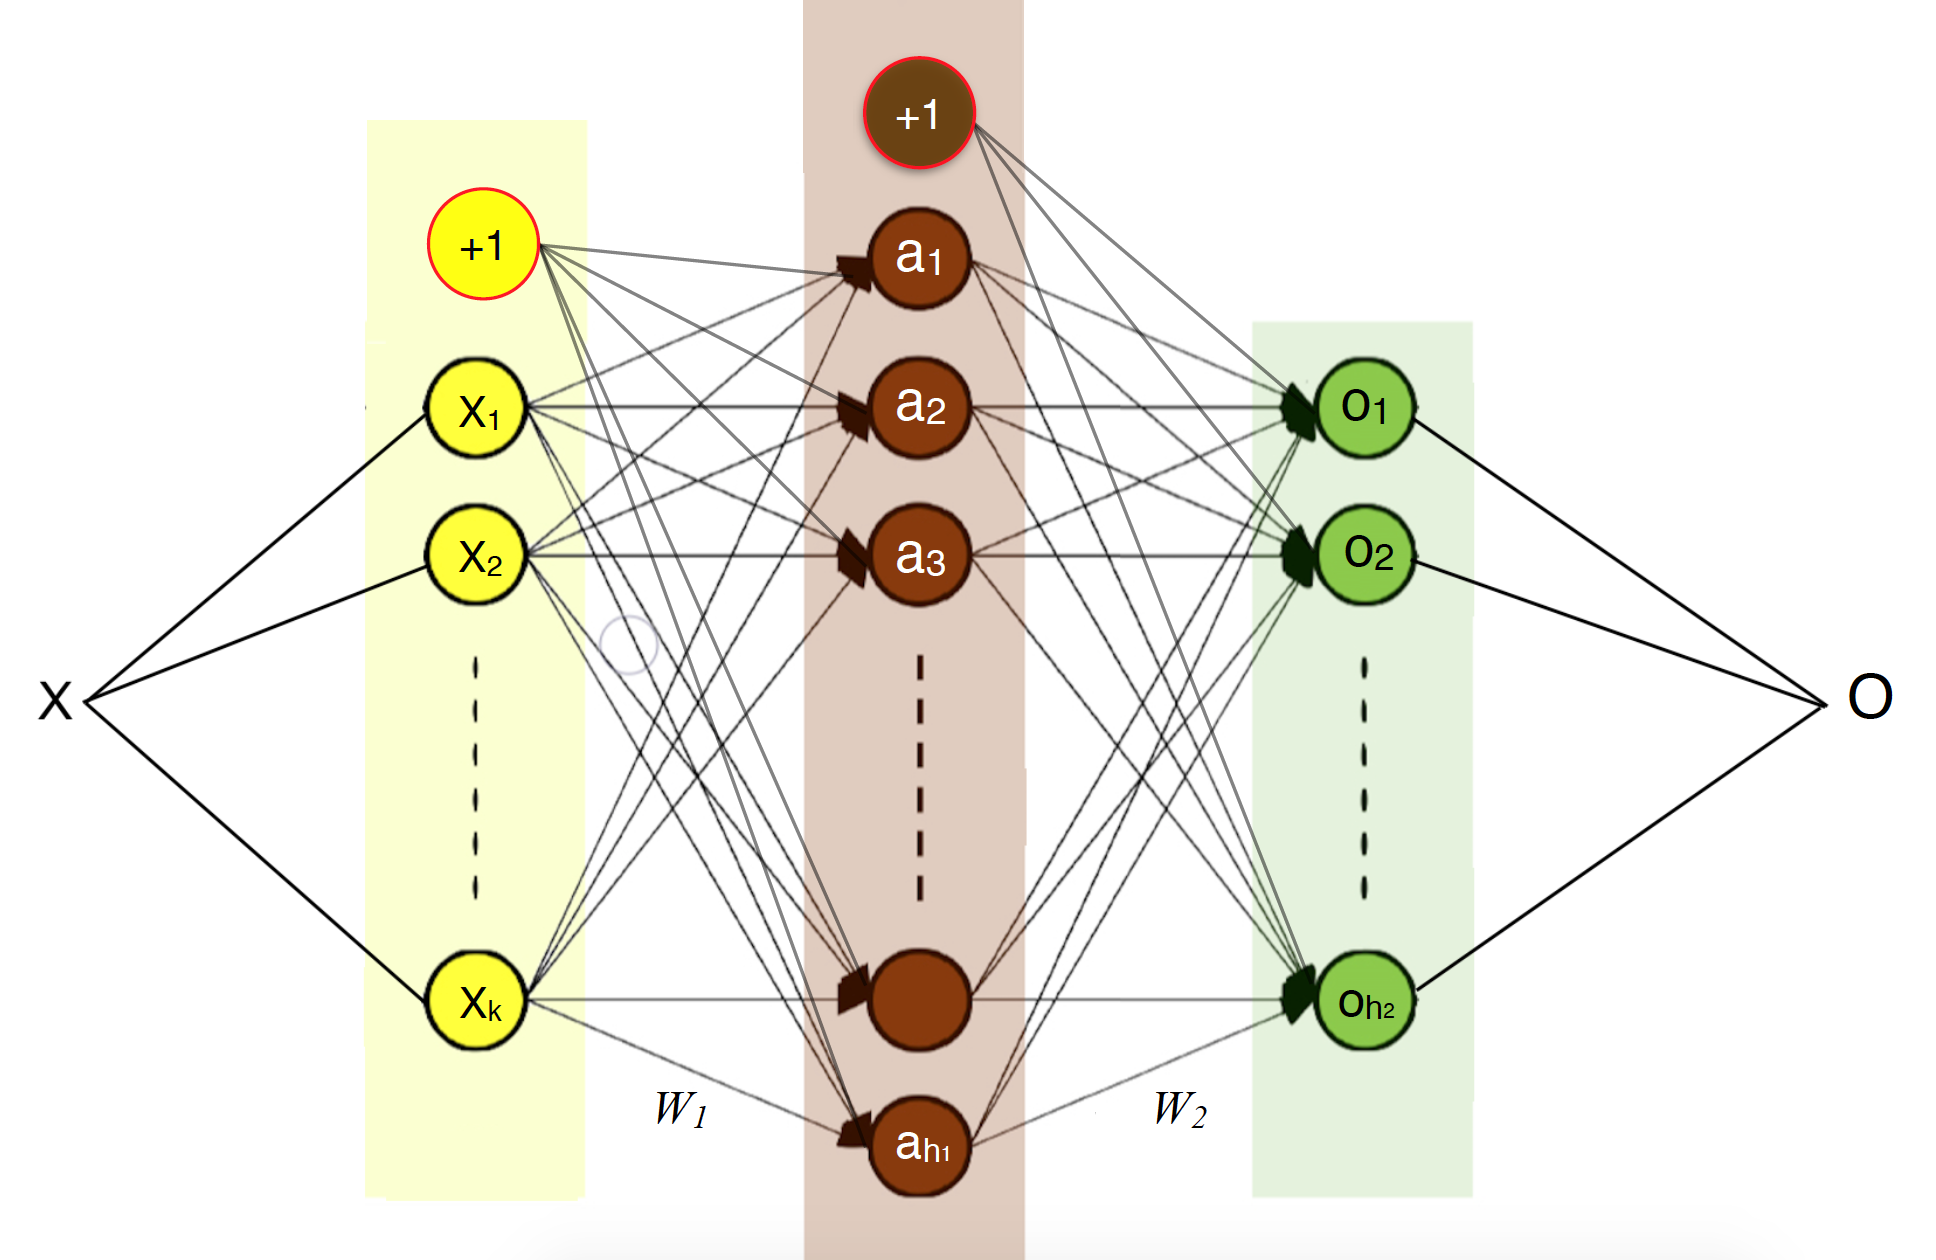
\includegraphics[width = 0.9\textwidth]{plots/revised_nn.png}
\end{center}
\end{figure}

The output of the network can be written as a function of the neural network parameters:
\begin{align*}
	f = \underbrace{S(\underbrace{\underbrace{g(\underbrace{xW_1 + b_1}_{f_1})}_{a}W_2 + b_2}_{f_2})}_{o}
\end{align*}

The specifications of the network are as follows:
\begin{itemize}
\item $x$ is a single data point of shape $1 \times k$. 
\item $g$ is an activation function - either the \textbf{sigmoid} or the \textbf{tanh} function for the purposes of this problem.
\item $S$ is the softmax function.
\item $h_{1}$ is the number of hidden units in layer 1 and $h_{2}$ is the number of hidden units in layer 2. 
\item $f$ is the output matrix of shape $1 \times h_{2}$.
\item $a$, $o$ are the activations of the hidden and output layer, of shapes $1 \times h_1$ and $1 \times h_2$, respectively.
\item $W_{1}$, $W_{2}$ are weight matrices of shape $k \times h_{1}$ and $h_{1} \times h_{2}$,  respectively.
\item $b_{1}$, $b_{2}$ are bias vectors of shape $1 \times h_{1}$ and $1 \times h_{2}$, respectively.
\end{itemize}

\pagebreak

So, we have that:
\begin{tabbing}
\hspace*{2cm}\=\hspace*{3cm}\= \kill
 \hspace*{10mm} $f_1 =$ \> $xW_1+b_1$ \> shape $1 \times h_1$, the linear combination output $f_1$ of $x$ using $W_1$\\
 \hspace*{10mm} $a =$ \> $g(f_1)$ \> shape $1 \times h_1$, the nonlinear activation function output $a$\\
 \hspace*{10mm} $f_2 =$ \> $aW_2+b_2$ \> shape $1 \times h_2$, the linear combination output $f_2$ of $a$ using $W_2$\\
 \hspace*{10mm} $o =$ \> $S(f_2)$ \> shape $1 \times h_2$, the softmax output $o$ of $f_2$\\
\end{tabbing}

In this problem, we will consider neural networks constructed using the following two types of non-linear activation functions: 
\begin{itemize}
\item \textbf{sigmoid} $\sigma(x)$ = $\frac{1}{1 + e ^{-x}}$
\item \textbf{tanh} tanh(x) = $\frac{e^{2x}-1}{e^{2x}+1}$
\item \textbf{softmax} $S_i(x)$ = $\frac{e^{x_i}}{\sum_j{e^{x_j}}}$
\end{itemize}

\hfill \linebreak
Furthermore, we will use the Cross Entropy Loss given by:
\begin{equation*}
	Error(network) = -\sum_{i = 1}^{ {h_2}} y_i\log y'_i,
\end{equation*}
where $y_i$ $\in\{0,1\}$ is the target label, and $y'_i$ is the $i^{\text{th}}$ predicted output of the network.
\newline\newline

\subsection*{3.1 Reveal the Black box [20 pts]}
Derive the backpropagation algorithm with respect to the adjustable parameters of this network, using (a) \textbf{sigmoid $\sigma(x)$} as the activation function and (b) \textbf{tanh} as the activation function. Note: consider softmax activation for layer 2 in both cases (a) and (b). 

\begin{soln}
    % Type solution here
\end{soln}

\subsection*{3.2 Neural Networks Meet Logistic Regression [5 pts]}
Recall that Logistic Regression models the conditional probability of a label $Y\in\{0,1\}$ given $p$-dimensional input $X\in\mathbb{R}^{p}$ as:
\begin{equation*} \label{eq:prob1}
P(Y=0|X=x)=\frac{1}{1 + \exp(w^T x)}
\end{equation*}
and
\begin{align*}
P(Y=1|X=x) &= 1- P(Y=0|X=x)\\
&= \frac{\exp(w^T x)}{1 + \exp(w^T x)},
\end{align*}
where $w\in \mathbb{R}^{p}$ denotes a weight vector.\newline\newline
Using only sigmoid and linear activation functions, create a Neural Network that for a three-dimensional input $X\in\mathbb{R}^{3}$  behaves like an ensemble of two Logistic Regression classifiers. Note that a Linear Activation function has the form $L(x) = C \, (w^T \, x)$, where $x$ is an input vector, $w$ is a weight vector, and $C$ is a constant; and by ensemble of classifiers here we simply mean a weighted linear combination of classifiers.

\begin{soln}
    % Type solution here
\end{soln}



